Resumen de diferentes partes: 

- Ajuste de agentes -> LoRa? -> comentar lo de los agentes instruct.
- El protocolo MCP
- El estado del arte en arquitecturas de agentes LLM y sistemas RAG
- 
- El estado del arte en agentes integrados a proyectos software + contexto de onboarding ~quizás en la introducción.
- Redes neuronales?

2. Agentes LLM (Fundamentos y funcionamiento básico)

¿Qué son los agentes LLM?
2.1. Modelos LLM
2.2. Interacción con herramientas
2.3. Abstracciones en frameworks


\section{Agentes LLM}

Los agentes de Inteligencia Artificial son programas informáticos que implementan modelos computacionales para ejecutar diversas funciones específicas del contexto en el que se aplican. Tras siete décadas y media de investigación, los esfuerzos en el campo se han focalizado en agentes basados en Grandes Modelos de Lenguaje (LLM). 

\subsection{Modelos LLM}

Los LLM son redes neuronales especializadas en el procesamiento del lenguaje natural, basados en la arquitectura Transformer. Esta arquitectura se fundamenta en el mecanismo de atención, el cual transforma la representación del texto para incorporar información contextual de manera escalable al hardware. 

Para comprender el funcionamiento de estos agentes, resulta imprescindible asimilar previamente conceptos como la tokenización y las representaciones vectoriales del lenguaje.

\paragraph{Tokens}
Los tokens constituyen la unidad mínima de texto que el modelo puede procesar. Dado que dichos modelos operan sobre estructuras matemáticas, requieren transformar el lenguaje natural en representaciones matriciales. Para lograr esta conversión, el texto se segmenta en dichas unidades mínimas, que pueden corresponder a caracteres individuales, fragmentos de texto o palabras completas. El conjunto íntegro de estas unidades reconocibles por el modelo configura su vocabulario. 

\paragraph{Representaciones vectoriales}
Constituyen vectores numéricos de dimensionalidad fija que codifican la semántica inherente a cada token. Estos vectores pueden comprender desde 768 dimensiones en arquitecturas como BERT-base hasta superar las 16.000 dimensiones en los modelos más avanzados del estado del arte. Por ejemplo, una dimensión específica podría especializarse en representar conceptos abstractos. En este contexto, la representación vectorial del token ``animal`` contendría un valor más elevado en dicha dimensión que la correspondiente al término ``gato``, reflejando su mayor grado de abstracción conceptual.


\subsection{Interacción con herramientas externas}
Los agentes LLM poseen la capacidad de interactuar con diversas herramientas como búsquedas web, bases de datos o interfaces de usuario. Fundamentalmente, un LLM solo genera tokens de texto, por lo que la integración de herramientas se implementa mediante palabras clave que el modelo puede incluir en su salida. Para ello, en el texto de entrada se especifica el esquema de la función a utilizar y, si decide emplearla, el modelo generará el texto correspondiente. Posteriormente, se procesa la respuesta para extraer llamadas a funciones si las hubiese.

La interacción con herramientas es típicamente alternante. Tras realizar la llamada a la herramienta, la salida de esta se utilizará como entrada para el siguiente mensaje del modelo. La figura \ref{fig:herramientas} ilustra el esquema de un agente con acceso a una API del clima. Como el modelo carece de información climática en tiempo real, se le indica en el prompt la posibilidad de invocar esta función. Al incluir la llamada en su texto de salida, se ejecuta la función y su respuesta se transmite al modelo para generar el resultado final.

\begin{figure}
  \centering
  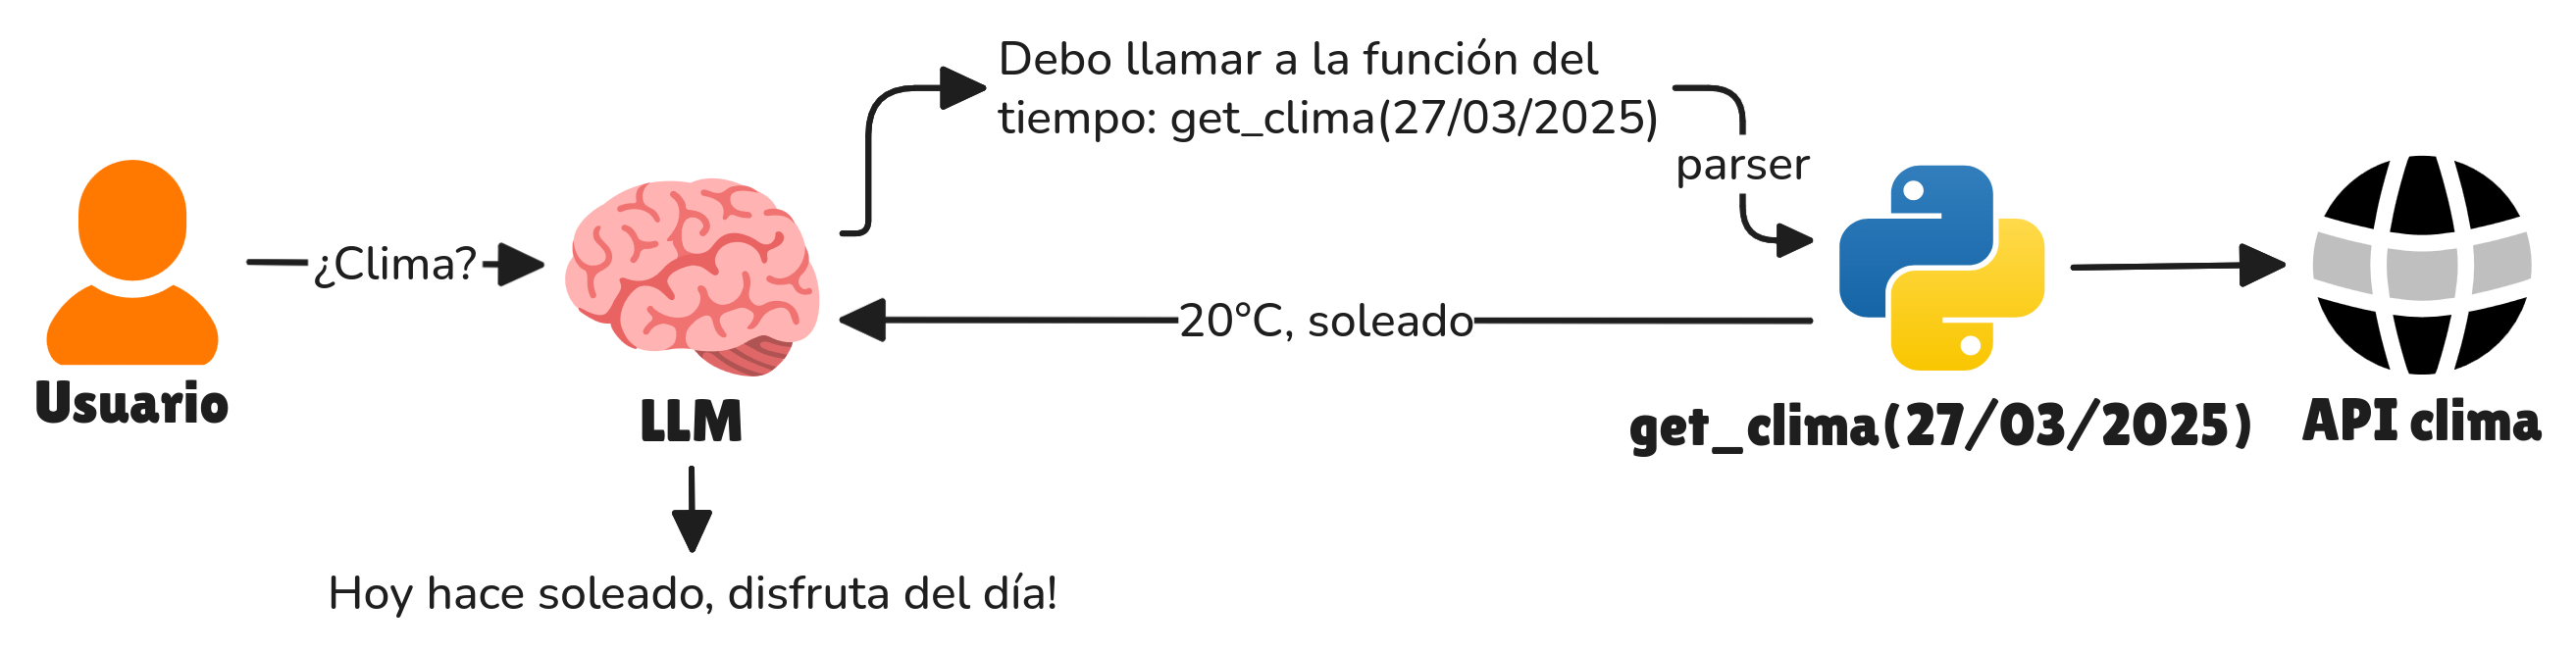
\includegraphics[width=1\linewidth]{figures/herramienta.png}
  \caption{Ejemplo de interacción de un modelo LLM con una herramienta externa.}
  \label{fig:herramientas}
\end{figure}

\subsection{Abstraciones en frameworks}
Aunque los agentes LLM son una tecnología de reciente surgimiento, ya se han desarrollado frameworks que estandarizan su implementación. Estas estructuras de trabajo, como LangChain o LangGraph, ofrecen abstracciones de alto nivel para reutilizar funcionalidades comunes presentes en la mayoría de sistemas de agentes.
Las funcionalidades principales que estos frameworks proporcionan son:
\begin{itemize}
\item {\textbf{Gestión de modelos:}} La ejecución de LLM requiere dominio del modelo empleado, ya que cada uno posee tokenizadores específicos y esquemas propios de entrada/salida. Los frameworks ofrecen interfaces unificadas, facilitando el uso de diversos modelos sin conocimientos técnicos precisos.
\item {\textbf{Interacción conversacional:}} La comunicación con los modelos se efectúa mediante un esquema conversacional, donde el modelo recibe un texto de entrada y genera una respuesta correspondiente. Las respuestas y entradas se concatenan secuencialmente para preservar el contexto de la conversación, cada consulta subsiguiente incorpora todos los intercambios precedentes.
  \item {\textbf{Uso de herramientas externas:}} El desarrollador únicamente debe especificar la función que desea incorporar, toda la compljeidad de la interacción se abstrae en el framework.
\item {\textbf{Interacción entre agentes:}} Los agentes pueden establecer comunicación entre sí, permitiendo la construcción de sistemas con mayor complejidad. Algunos frameworks establecen protocolos que definen las modalidades de comunicación entre los distintos agentes.
\end{itemize}

\section{Model Context Protocol}
todo: referencias a las docs.

El Model Context Protocol (MCP), desarrollado por Anthropic, estandariza la comunicación entre agentes LLM y herramientas. Permite que aplicaciones diversas ofrezcan herramientas a agentes externos sin exponer detalles de implementación. Comparable al modelo OSI, el MCP opera en un nivel de abstracción inferior a los frameworks, proporcionando una capa de interoperabilidad.

La figura \ref{fig:mcp} ilustra el esquema operativo del protocolo. En este contexto, los desarrolladores de Jira y GitHub han implementado un servidor MCP que proporciona las herramientas disponibles al cliente MCP. Este servidor realiza la traducción de las interacciones necesarias con las API de Jira y GitHub, permitiendo que el agente LLM únicamente requiera conocer el esquema funcional que debe utilizar. Por su parte, el cliente MCP se encarga de administrar la comunicación con los diferentes servidores, facilitando que el agente acceda directamente a las herramientas disponibles.

\begin{figure}
  \centering
  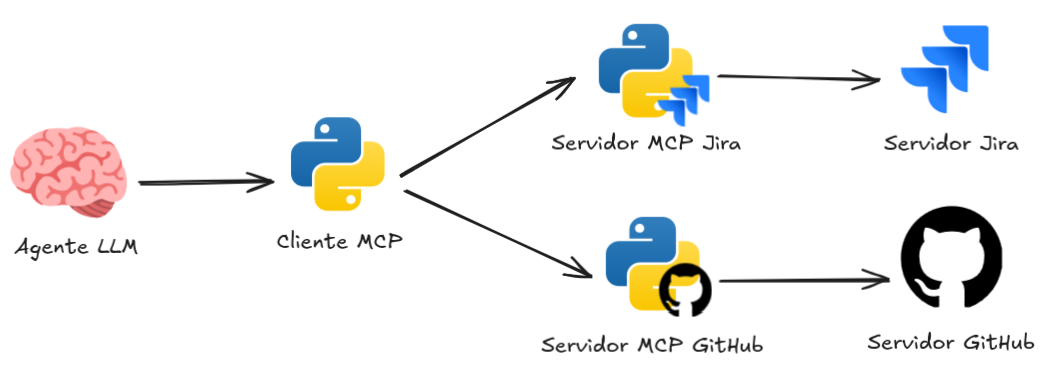
\includegraphics[width=1\linewidth]{figures/mcp.png}
  \caption{Esquema de funcionamiento del Model Context Protocol.}
  \label{fig:mcp}
\end{figure}


El protocolo ofrece dos modos de operación para establecer la comunicación entre cliente y servidor:
\begin{itemize}
  \item{\textbf{Comunicación SSE: } El protocolo Server-Sent Events (SSE) establece un canal de comunicación unidireccional sobre HTTP desde el servidor hacia el cliente. Proporciona actualizaciones en tiempo real con capacidad de streaming. En el protocolo MCP, el cliente efectúa solicitudes para la ejecución de herramientas en el servidor mediante HTTP, a lo que el servidor puede responder mediante eventos SSE.}
\item{\textbf{Comunicación STDIO: } El protocolo de entrada y salida estándar (STDIO) facilita la comunicación bidireccional entre cliente y servidor a nivel de proceso en el sistema operativo. Este mecanismo permite el intercambio de información en formato JSON a través de los canales estándar del sistema. Su diseño, orientado principalmente a entornos locales, restringe la conexión a un único cliente por servidor al limitarse a la comunicación entre dos procesos.}
\end{itemize}
La aplicación de escritorio claude-desktop de Anthropic constituye un reflejo del potencial del protocolo. Esta plataforma ofrece la posibilidad de interactuar con servidores preconfigurados mediante una configuración mínima. Implementando el protocolo STDIO, la aplicación ejecuta los servidores distribuidos por terceros a través del gestor de paquetes UV o Docker. Al incorporar un cliente MCP en la aplicación, consigue integrar las herramientas disponibles en la interfaz de chat con los modelos de Anthropic.

\section{Estado del arte en arquitecturas de agentes LLM}

La comunidad científica ha desarrollado diferentes arquitecturas de agentes para sacar el máximo provecho al rendimiento de los modelos disponibles. Es de destacar la arquitectura RAG, la cual complementa la entrada del modelo con la recuperación de documentos relevantes. Por otro lado, se han realizado diversos esfuerzos en investigar diferentes arquitecturas de comunicación, estrategias de planning o sistemas de memoria, entre otros.

\subsection{Arquitectura RAG}

Los modelos LLM poseen un conocimiento restringido a los datos con los que fueron entrenados. Para superar esta limitación, la arquitectura RAG (Retrieval-Augmented Generation) complementa la generación del LLM mediante la recuperación de información relevante desde repositorios de conocimiento externos. La figura x ilustra un ejemplo de su funcionamiento.    

La recuperación de documentos relevantes se implementa mediante diversas estrategias: expresiones regulares, búsqueda de trigramas [ref], palabras clave, entre otras. No obstante, el enfoque predominante consiste en la indexación vectorial. En este método, los documentos se transforman en vectores, generalmente mediante LLMs especializados en codificación, denominados Embedders. Al representar los documentos en un espacio vectorial, es posible recuperar aquellos semánticamente más pertinentes mediante la comparación del vector de consulta con los vectores de los documentos indexados, utilizando métricas como la distancia coseno.

\subsubsection{Estrategias RAG avanzadas}
La mejora del rendimiento de la arquitectura RAG ha sido objeto de extensa investigación \cite{zhu_retrieving_2021}\cite{gao_retrieval-augmented_2024}. La optimización de esta estrategia se ha centrado en mejorar el procesado de documentos, sistemas de extracción, sistemas de recuperación y optimización del pipeline general: 


\begin{itemize}
  \item {\textbf{procesado de documentos:}} El procesado previo a la indexación de documentos determina la calidad de la información. Entre las estrategias más destacadas se encuentran optimizaciones como limpiar el ruido de los documentos, la optimización del tamaño de chunks para el embedder utilizado, o el sistema overlapping window, el cual consiste en superponer los chunks para evitar la pérdida de información en los límites de los mismos. 

    Adicionalmente, se han desarrollado técnicas de generación para mejorar la calidad de los documentos. Estas técnicas varían desde recuperar documentos directamente generados\cite{yu_generate_2023}, recitar pasajes de evidencia\cite{sun_recitation-augmented_2023}, o utilizar un documento generado a partir de la query para buscar documentos relevantes\cite{gao_precise_2023}. Estas técnicas se pueden combinar con el algoritmo beam search para más efectividad\cite{cheng_lift_nodate}.

\item {\textbf{sistemas de extracción:}}
\item {\textbf{sistemas de recuperación:}} 
\item {\textbf{optimización del pipeline:}} 
\end{itemize}



\subsection{Arquitecturas de interacción entre agentes}
La interacción entre agentes LLM es también un campo de investigación activo. 










